\documentclass[a4paper,12pt]{article}
    \usepackage{listing}
    \usepackage{graphicx}
    
    \begin{document}
        
    \title{Concurrent Time Server}
    \author{Santhisenan A}
    \date{\today}
    \maketitle
        
    \section{Socket programming}
        
    % \subsection{some title here}
    Sockets can be thought of as endpoints in a communication channel that is 
    bi-directional, and establishes communication between a server and one or 
    more clients. Here, we set up a socket on each end and allow a client to interact 
    with other clients via the server. The socket on the server side associates itself 
    with some hardware port on the server side. Any client that has a socket associated
    with the same port can communicate with the server socket.
        
    \section{Multi-Threading}
    
    
    
    A thread is sub process that runs a set of commands individually of any other thread.
    So, every time a user connects to the server, a separate thread is created for that user
    and communication from server to client takes place along individual threads based on
    socket objects created for the sake of identity of each client.
    We will require two scripts to establish this chat room. One to keep the serving running,
    and another that every client should run in order to connect to the server.
    
    \section{Code}
    \subsection{Server}
    \begin{verbatim}
        import socket
        import time
        
        UDP_IP = "127.0.0.1"
        UDP_PORT = 5005
        
        sock = socket.socket(socket.AF_INET, # Internet
                             socket.SOCK_DGRAM) # UDP
        sock.bind((UDP_IP, UDP_PORT))
        
        while True:
            # ClientSocket, addr = sock.accept()
            message, ClientSocket = sock.recvfrom(1024) # buffer size is 1024 bytes
            CurrentTime = time.ctime(time.time()) + "\r\n"
            sock.sendto(CurrentTime.encode('ascii'),ClientSocket)
            # sock.close()
    \end{verbatim}

    \subsection{Client}
    \begin{verbatim}
        import socket

        UDP_IP = "127.0.0.1"
        UDP_PORT = 5005
        MESSAGE = "Hello, World!"
        
        print "UDP target IP:", UDP_IP
        print "UDP target port:", UDP_PORT
        # print "message:", MESSAGE
        sock = socket.socket(socket.AF_INET, # Internet
                             socket.SOCK_DGRAM) # UDP
        sock.sendto(MESSAGE, (UDP_IP, UDP_PORT))
        message, ServerAddress = sock.recvfrom(1024)
        print "Time revceived: ", message        
    \end{verbatim}
    \section{Output}
    \pagebreak
    
    \begin{figure}
        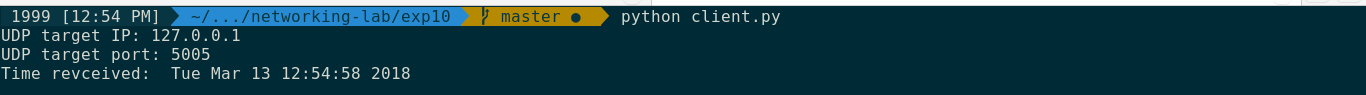
\includegraphics[width=\linewidth]{./timeserver.png}
        \caption{Client}
        \label{fig:client}
    \end{figure}

    
    
    \end{document}